\section{Introduction}

This chapter presents the experimental results of the proposed explainable transfer learning framework for skin condition classification and severity estimation. Three pre-trained convolutional neural network (CNN) architectures---EfficientNetB0, MobileNetV2, and ResNet50---were evaluated under four dataset split configurations. The models were assessed using Accuracy, Precision, Recall, F1-score, ROC-AUC, and inference time per image. Grad-CAM was also employed to visualize image regions associated with model predictions. The results are presented through quantitative evaluation, comparative analysis, and qualitative examination of model explanations.

\section{Experimental Setup}

The experiments used a processed skin condition dataset containing 8,275 images categorized into four main groups: Acne, Burn, Eczema, and Normal skin. These groups were represented by 12 labels, comprising mild, moderate, and severe levels for Acne, Burn, and Eczema, together with dry, normal, and oily skin types.

Four dataset split configurations were considered: 60:20:20, 70:15:15, 80:10:10, and 90:5:5, representing the percentages allocated to training, validation, and testing, respectively. Each of the three CNN architectures was associated with these four configurations, resulting in twelve model configurations.

The model names follow the convention \texttt{architecture\_train\_validation\_test}. For example, \texttt{resnet50\_90\_5\_5} denotes ResNet50 with 90\% of the data allocated to training, 5\% to validation, and 5\% to testing.

Model performance was assessed using Accuracy, Precision, Recall, F1-score, and ROC-AUC. Inference time per image was measured to compare computational efficiency. Grad-CAM visualizations were generated to examine the image regions associated with model predictions.

\section{Training Performance}

The training and validation accuracy and loss curves were examined to assess the learning behavior of the twelve model configurations. Accuracy curves provide information about changes in classification performance during training, whereas loss curves help illustrate the optimization process. Differences between training and validation behavior can also provide indications of potential overfitting.

Figure~\ref{fig:training_validation_accuracy_curve} presents the training and validation accuracy curves, while Figure~\ref{fig:training_validation_loss_curve} shows the corresponding loss curves.

\begin{figure}[htbp]
\centering
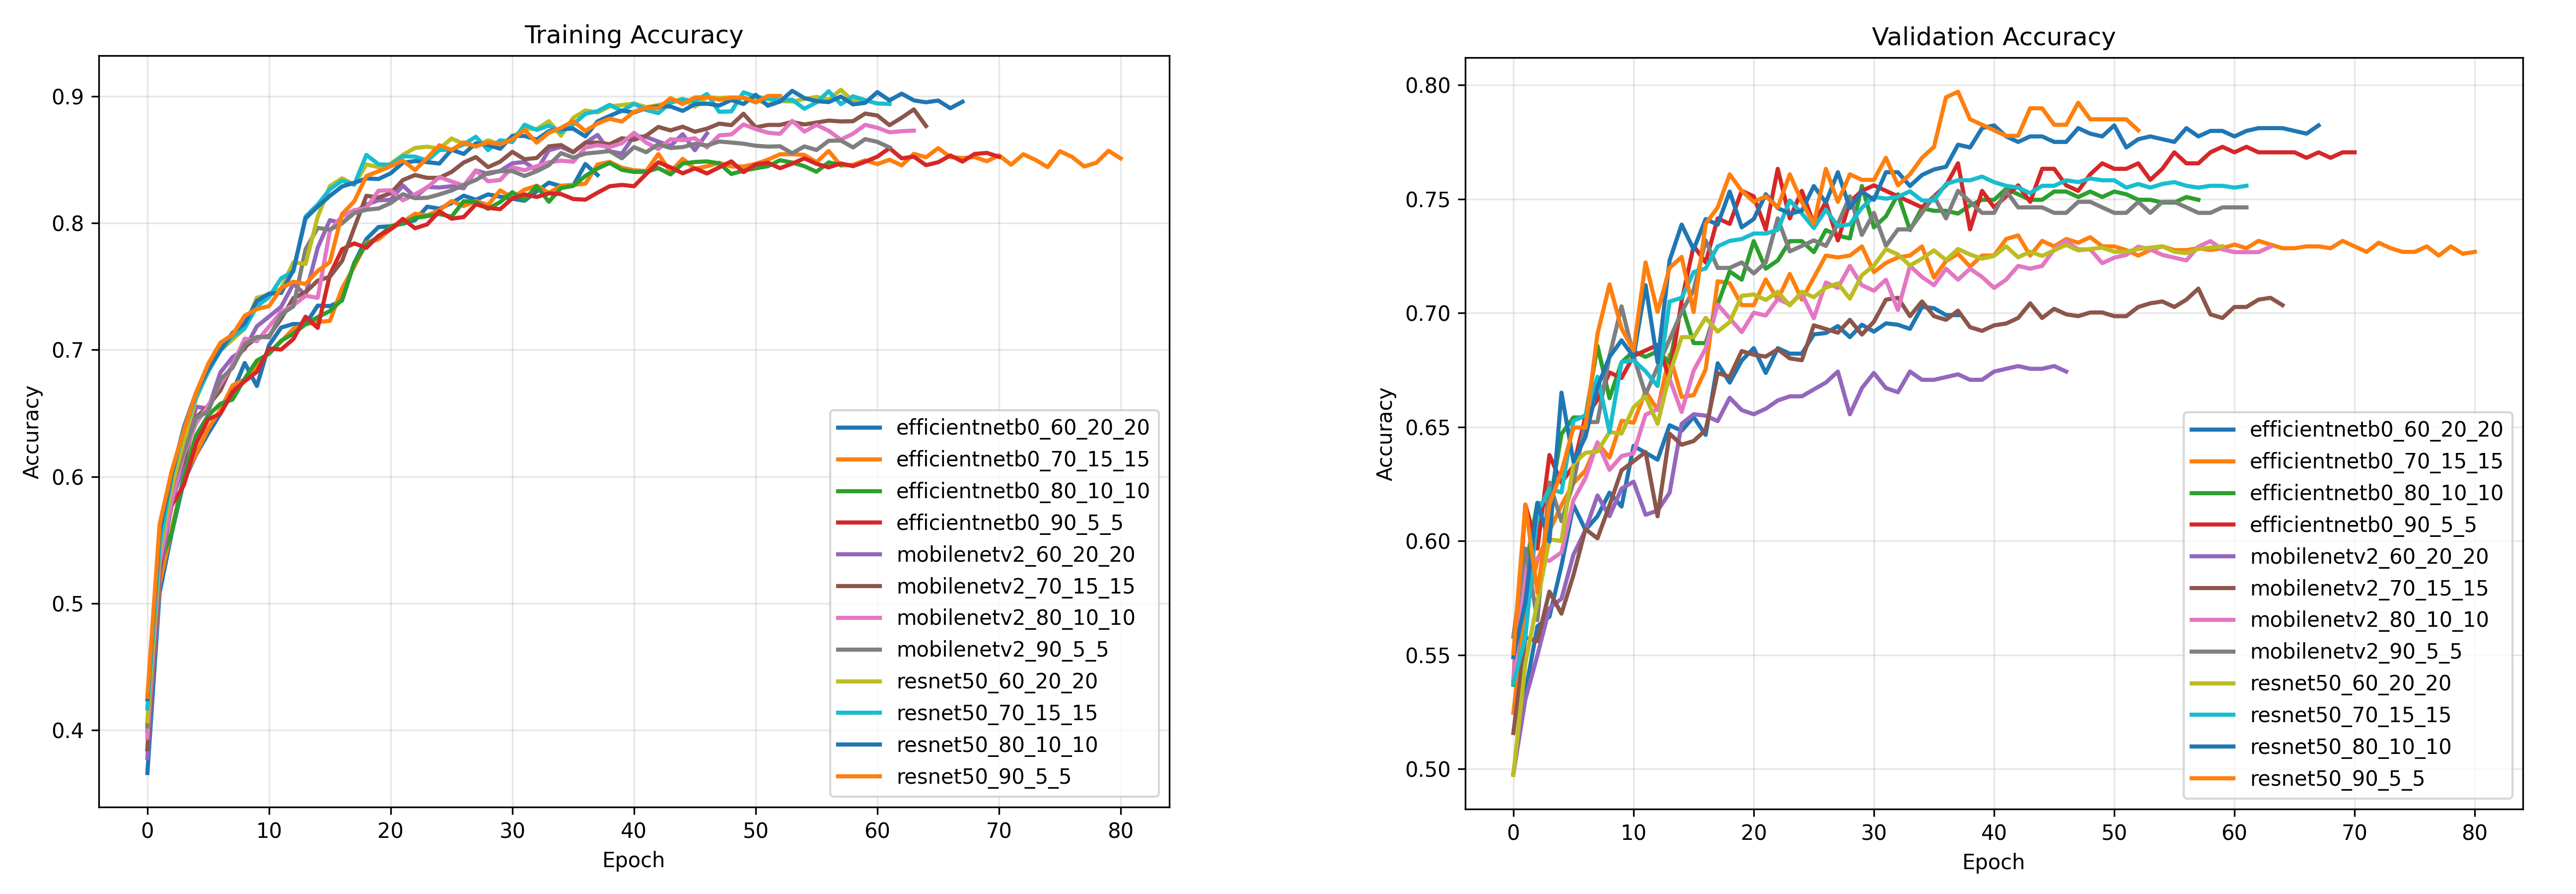
\includegraphics[width=0.85\textwidth]{images/training-curve.png}
\caption{Training and Validation Accuracy Curves}
\label{fig:training_validation_accuracy_curve}
\end{figure}

\begin{figure}[htbp]
\centering
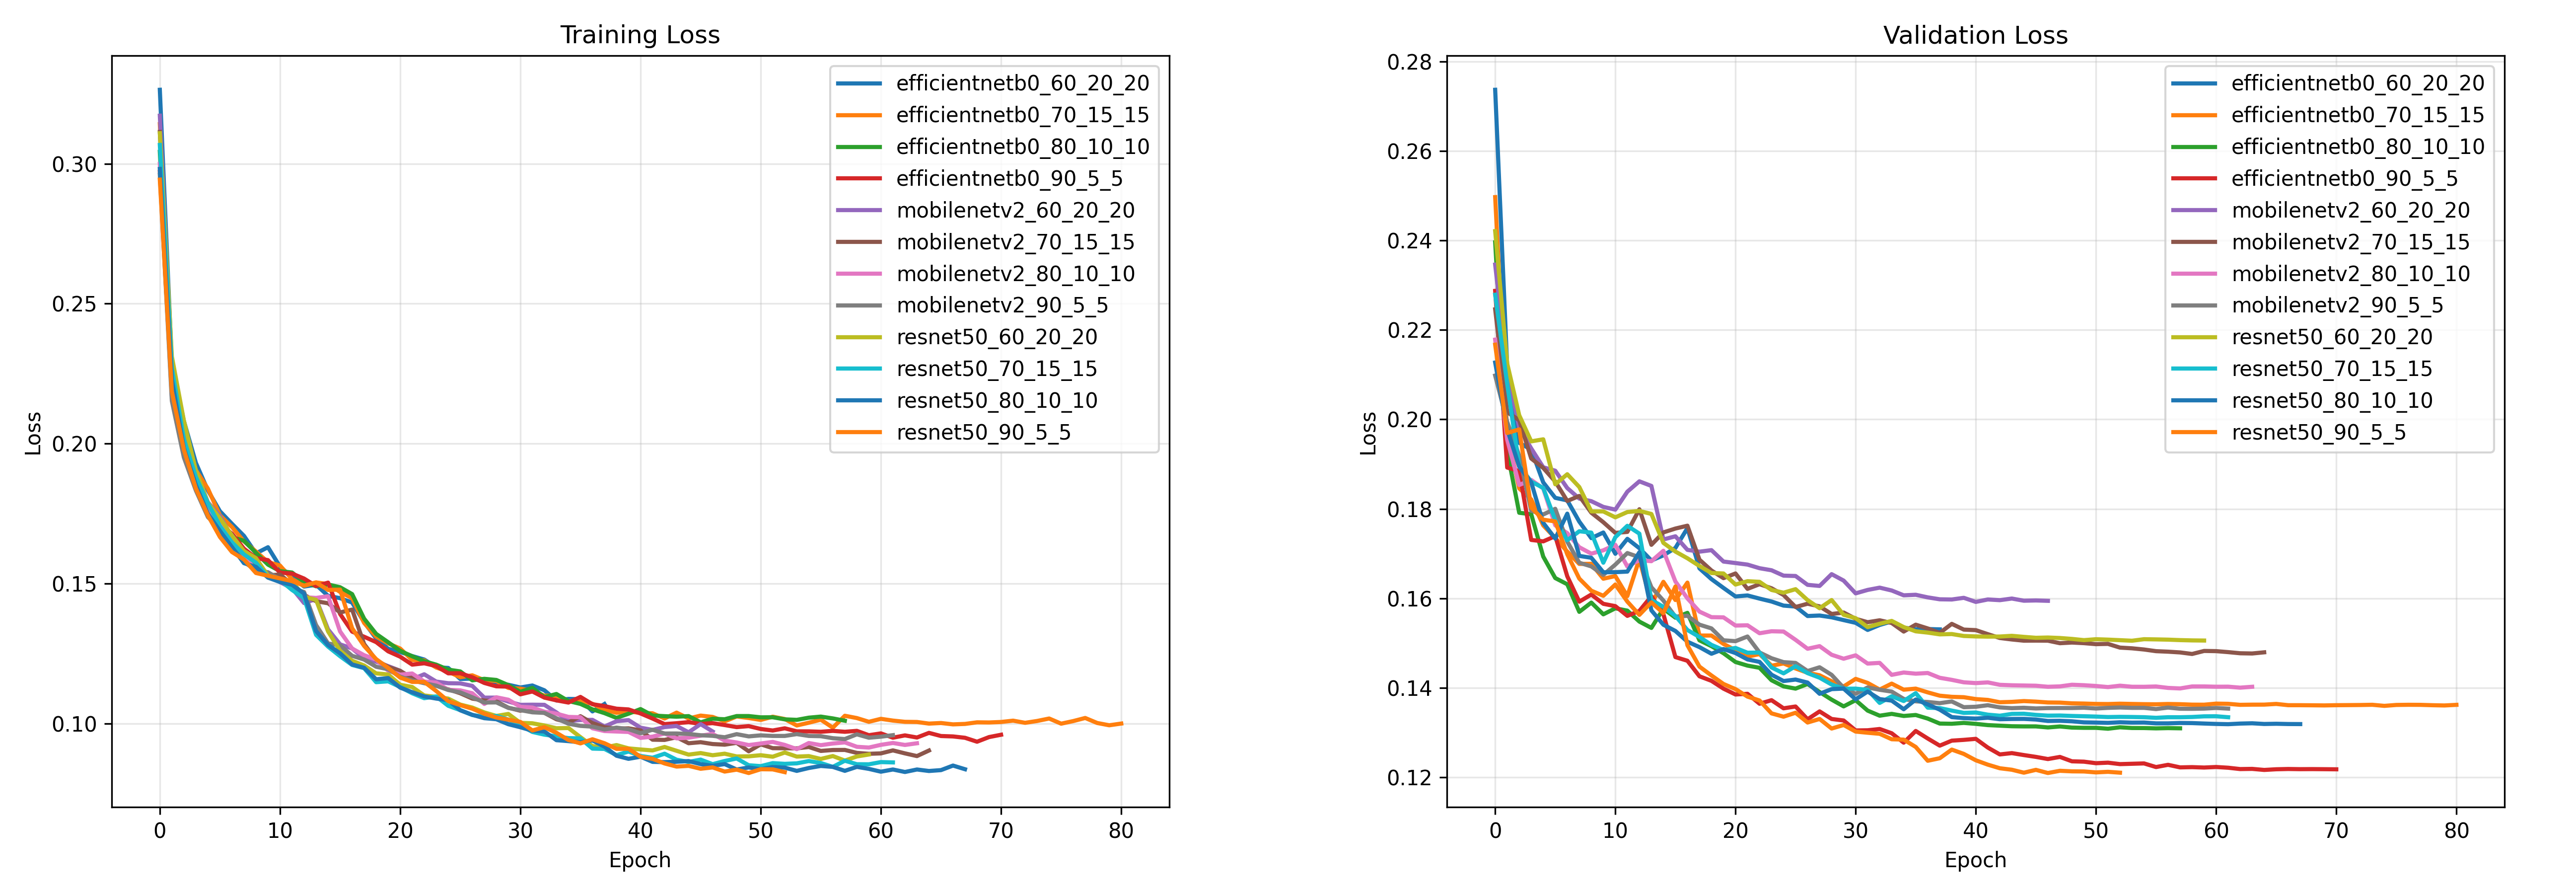
\includegraphics[width=0.85\textwidth]{images/loss-curve.png}
\caption{Training and Validation Loss Curves}
\label{fig:training_validation_loss_curve}
\end{figure}

The learning behavior of each model should be interpreted in relation to its architecture and dataset split. A larger training partition provides more examples for learning discriminative features, while the validation partition supports monitoring and model selection. However, training curves alone are insufficient to establish generalization performance. The quantitative evaluation and the validity of the test procedure must also be considered when comparing the models.

\section{Performance Evaluation}

All twelve models were compared using Accuracy, Precision, Recall, F1-score, ROC-AUC, and inference time per image. The reported results are presented in Table~\ref{tab:model_comparison}.

\begin{table}[htbp]
\centering
\resizebox{\textwidth}{!}{%
\begin{tabular}{|l|c|c|c|c|c|c|}
\hline
\textbf{Model} &
\textbf{Accuracy (\%)} &
\textbf{Precision (\%)} &
\textbf{Recall (\%)} &
\textbf{F1-score (\%)} &
\textbf{ROC-AUC (\%)} &
\textbf{Inference Time (ms/image)} \\
\hline
EfficientNetB0\_60\_20\_20 & 69.81 & 69.89 & 69.81 & 69.62 & 96.67 & 26.13 \\
\hline
EfficientNetB0\_70\_15\_15 & 73.19 & 73.44 & 73.19 & 72.94 & 97.26 & 24.26 \\
\hline
EfficientNetB0\_80\_10\_10 & 74.88 & 74.98 & 74.88 & 74.70 & 97.49 & 26.16 \\
\hline
EfficientNetB0\_90\_5\_5 & 85.02 & 85.17 & 85.02 & 84.88 & 98.94 & 23.27 \\
\hline
MobileNetV2\_60\_20\_20 & 67.03 & 67.49 & 67.03 & 66.83 & 96.59 & 16.36 \\
\hline
MobileNetV2\_70\_15\_15 & 71.62 & 71.88 & 71.62 & 71.46 & 97.33 & 16.15 \\
\hline
MobileNetV2\_80\_10\_10 & 73.91 & 74.04 & 73.91 & 73.59 & 97.54 & 16.54 \\
\hline
MobileNetV2\_90\_5\_5 & 83.21 & 83.71 & 83.21 & 83.16 & 98.72 & 18.53 \\
\hline
ResNet50\_60\_20\_20 & 72.83 & 73.16 & 72.83 & 72.43 & 97.23 & 55.82 \\
\hline
ResNet50\_70\_15\_15 & 76.09 & 76.37 & 76.09 & 75.81 & 97.91 & 54.03 \\
\hline
ResNet50\_80\_10\_10 & 78.50 & 78.97 & 78.50 & 78.34 & 98.02 & 66.58 \\
\hline
ResNet50\_90\_5\_5 & \textbf{86.84} & \textbf{87.22} & \textbf{86.84} & \textbf{86.79} & \textbf{99.27} & 72.42 \\
\hline
\end{tabular}%
}
\caption{Performance Comparison of All Twelve Transfer Learning Models}
\label{tab:model_comparison}
\end{table}

According to the reported results, \texttt{ResNet50\_90\_5\_5} achieved the highest values for Accuracy, Precision, Recall, F1-score, and ROC-AUC. Its results were 86.84\%, 87.22\%, 86.84\%, 86.79\%, and 99.27\%, respectively. Among the remaining configurations, \texttt{EfficientNetB0\_90\_5\_5} achieved an Accuracy of 85.02\%, while \texttt{MobileNetV2\_90\_5\_ 5} achieved 83.21\%.

The lowest reported Accuracy was 67.03\%, obtained by \texttt{MobileNetV2\_60\_20\_20}. The results therefore show variation in classification performance across both the CNN architectures and the dataset configurations.

Inference time also differed across the models. \texttt{MobileNetV2\_70\_15\_15} recorded the shortest time at 16.15 ms per image, whereas \texttt{ResNet50\_90\_5\_5} recorded the longest at 72.42 ms per image. These measurements indicate that classification performance and inference speed should be considered together when selecting a model for a particular application.

\section{Comparative Analysis}

This section compares EfficientNetB0, MobileNetV2, and ResNet50
across the four evaluated dataset split configurations:
60:20:20, 70:15:15, 80:10:10, and 90:5:5. The comparison considers
Accuracy, Precision, Recall, F1-score, ROC-AUC and inference time to examine
both classification performance and computational efficiency.
Figure~\ref{fig:model_comparison} provides a visual summary of these
metrics across the evaluated configurations.

\begin{figure}[htbp]
    \centering
    \includegraphics[width=\textwidth]{images/model-comparison.png}
    \caption{Comparison of EfficientNetB0, MobileNetV2, and ResNet50
    across four dataset split configurations in terms of
    (a) Accuracy, (b) Precision, (c) Recall, (d) F1-score, (e) ROC-AUC  and
    (f) inference time.}
    \label{fig:model_comparison}
\end{figure}

\subsection{Comparison Across Dataset Split Configurations}

The reported Accuracy increased across the four split configurations for each of the three architectures. For EfficientNetB0, Accuracy increased from 69.81\% under 60:20:20 to 74.88\% under 80:10:10, before reaching 85.02\% under 90:5:5. MobileNetV2 followed a similar pattern, increasing from 67.03\% to 73.91\% across the first three configurations and reaching 83.21\% under 90:5:5. ResNet50 increased from 72.83\% under 60:20:20 to 78.50\% under 80:10:10 and 86.84\% under 90:5:5.

This pattern suggests that the configurations with larger training proportions were associated with higher reported Accuracy. One possible explanation is that a larger training set provides more examples from which the model can learn useful image representations. Nevertheless, the observed differences cannot be attributed solely to the amount of training data without ensuring that the evaluation procedure is consistent across configurations.

The 90:5:5 configuration also allocates smaller proportions of the dataset to validation and testing. A smaller validation set may provide less information for model selection, while a smaller test set can lead to less stable performance estimates. Accordingly, the results do not establish that 90:5:5 is universally the best split configuration.

\subsection{Comparison of CNN Architectures}

The three architectures exhibited different balances between classification performance and inference time. ResNet50 achieved the highest reported Accuracy under each of the four split configurations. Its stronger reported classification performance was accompanied by longer inference times, particularly for the 90:5:5 configuration.

EfficientNetB0 provided a potential middle ground. Its \texttt{90\_5\_5} configuration achieved 85.02\% Accuracy with an inference time of 23.27 ms per image. Although this was lower in Accuracy than the corresponding ResNet50 configuration, its measured inference time was substantially shorter.

MobileNetV2 recorded the shortest inference times among the three architectures. Its fastest configuration, \texttt{MobileNetV2\_70\_15\_15}, required 16.15 ms per image. Its reported classification performance was lower than that of the corresponding EfficientNetB0 and ResNet50 configurations, but its speed may make it a useful candidate for applications with limited computational resources.

Overall, the reported results suggest that ResNet50 is a candidate when classification performance is the primary consideration, EfficientNetB0 may provide a compromise between performance and latency, and MobileNetV2 may be suitable where computational efficiency is particularly important. These conclusions should be considered provisional until the evaluation partitions are verified.

\section{Explainability Using Grad-CAM}

Gradient-weighted Class Activation Mapping (Grad-CAM) was incorporated to provide a qualitative view of the image regions associated with model predictions. It produces heatmaps using gradients associated with a target class, helping visualize which spatial regions contribute to the model's output.

\begin{figure}[htbp]
\centering
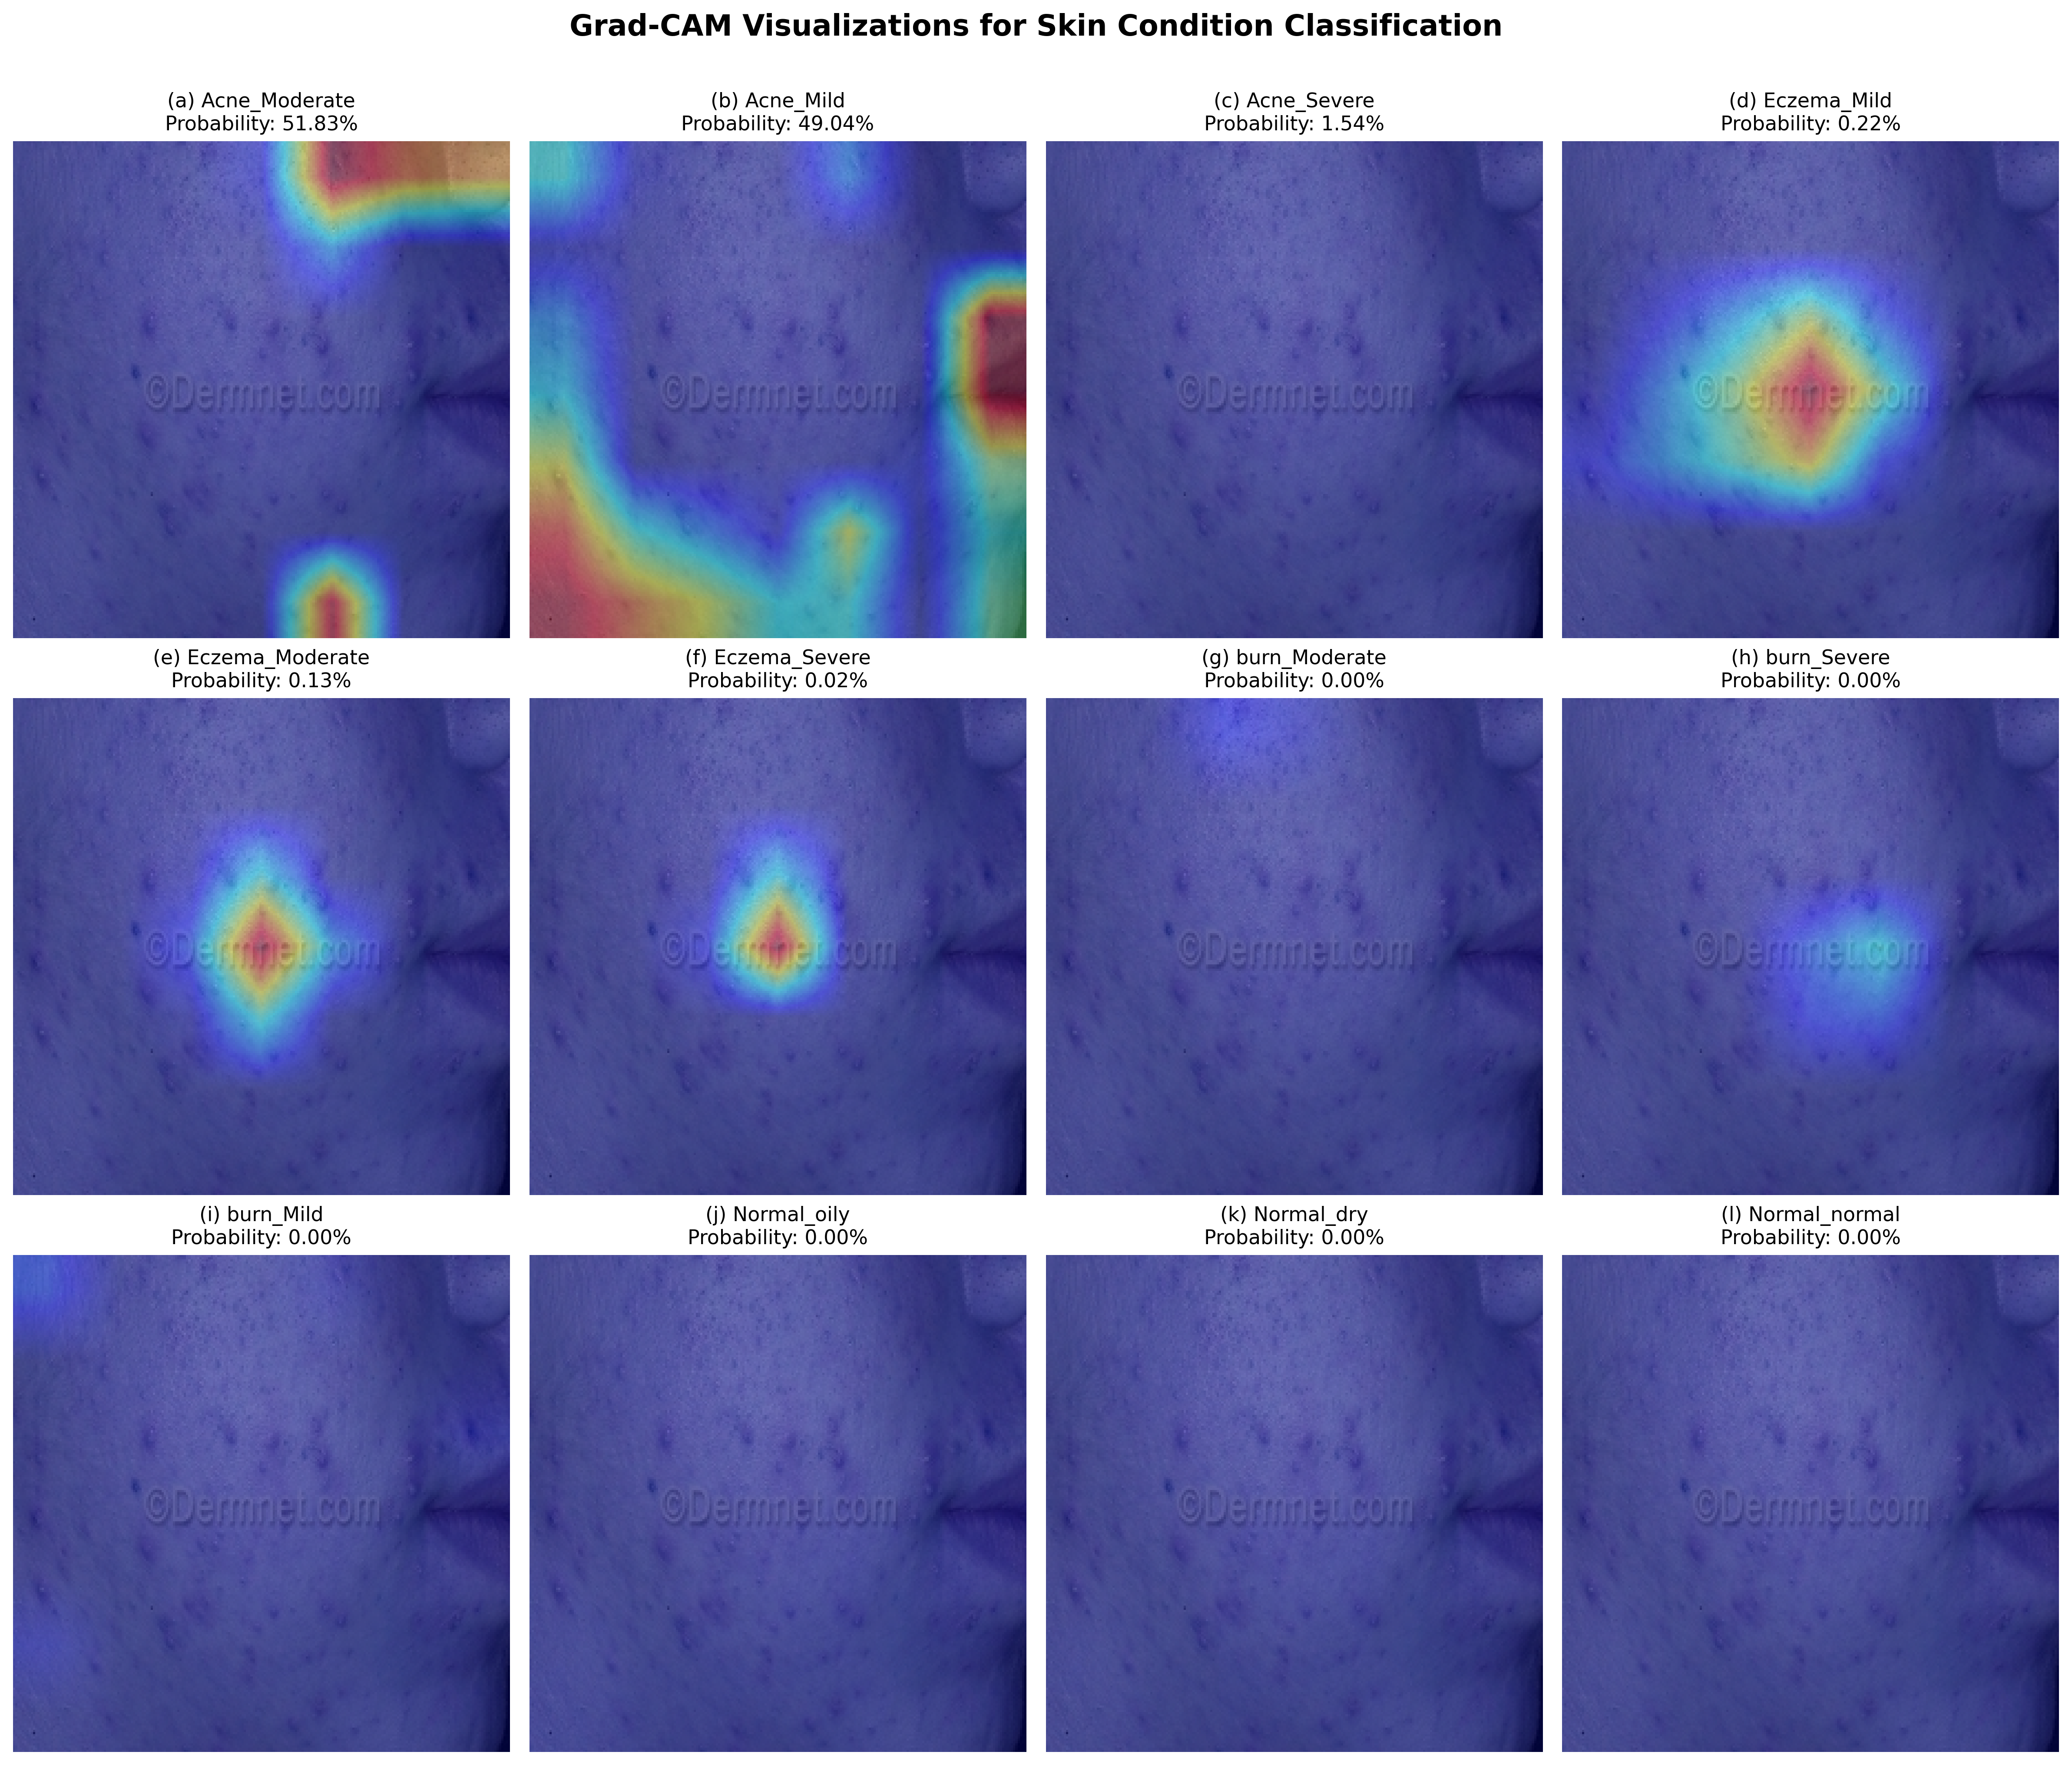
\includegraphics[width=0.85\textwidth]{images/gradcam_all_labels.png}
\caption{Grad-CAM Visualizations for Skin Condition Classification}
\label{fig:grad_cam_visualization}
\end{figure}

The generated heatmaps can be examined to determine whether the model's attention overlaps with relevant skin regions or appears to be influenced by background content. Features such as lesion boundaries, inflammation, and pigmentation should be discussed as observed findings only when the visualizations provide clear support for those interpretations.

Grad-CAM complements the quantitative evaluation by making aspects of model behavior easier to inspect. However, a heatmap does not prove that a model relies on clinically valid features or that its prediction is medically correct. These visualizations should therefore be interpreted as qualitative explanations rather than evidence of diagnostic validity.

\section{Discussion}

The results show differences among EfficientNetB0, MobileNetV2, and ResNet50 in classification performance and computational efficiency. \texttt{ResNet50\_90\_5\_5} achieved the highest reported Accuracy (86.84\%) and ROC-AUC (99.27\%), whereas \texttt{MobileNetV2\_70\_15\_15} recorded the shortest inference time (16.15 ms per image). These findings highlight the trade-off between classification performance and prediction speed when selecting a model.

Accuracy increased across the evaluated configurations as the training proportion increased. Although additional training images may help models learn more representative features, differences in validation and test set sizes may also affect the reported results. Therefore, the 90:5:5 configuration cannot be considered universally optimal based on these experiments alone.

Grad-CAM provides visual explanations of image regions associated with model predictions, but these visualizations do not establish clinical reliability. Further evaluation on diverse, independent datasets is needed to assess generalization and determine the framework's suitability for potential healthcare applications.

\section{Chapter Summary}

This chapter presented the reported results for twelve transfer learning configurations based on EfficientNetB0, MobileNetV2, and ResNet50. ResNet50\_90\_5\_5 achieved the strongest reported classification metrics, while MobileNetV2\_70\_15\_15 recorded the shortest inference time. The comparison illustrates the importance of balancing predictive performance with computational requirements. Grad-CAM was also used to support qualitative inspection of model predictions.

The principal methodological consideration is to verify that each model was evaluated on the appropriate independent test partition and that the evaluation metrics and inference times were calculated consistently. Resolving this issue is necessary before making definitive claims about the influence of dataset split proportions or selecting a model for practical deployment.